\chapter{\label{ch:intro} Introduction}

In the past decade, the integration of Augmented Reality (AR) into robotic systems has gained significant traction. Building upon this trend and previous work in robotics, this project aims to develop an innovative AR system for a wheeled robot. By combining AR technology with machine learning, we seek to enhance the robot's functionality and substantially improve the human-machine interaction experience. This fusion of technologies promises to push the boundaries of what's possible in robotic systems, offering new possibilities for both practical applications and user engagement.

%@@@@@@@@@@@@@@@@@@@@@@@@@@@@@@@@@@@@@@@@@@@@@@@@@@@@@@@@@@@@@@@@@@@@@@@@@@@@@@@@@@@@@@@@@@@@@@@@@@@@@@
\section{\label{sec:backg}Background}
The concept of autonomous vehicles dates back to the days of Leonardo Da Vinci's 16th-century designs, although practical implementations only emerged in the 1980s \cite{Mobileye2023}. Radio-controlled (RC) cars, introduced earlier by Elettronica \cite{RC_Crush2023}, evolved from combustion engines to electric motors, expanding their applications across various industries \cite{GoogleBooks2017}. As shown in Figure \ref{fig:davinci_car}, Da Vinci's early concept reflects humanity's long-standing fascination with autonomous transportation.

\begin{figure}[h]
\centering
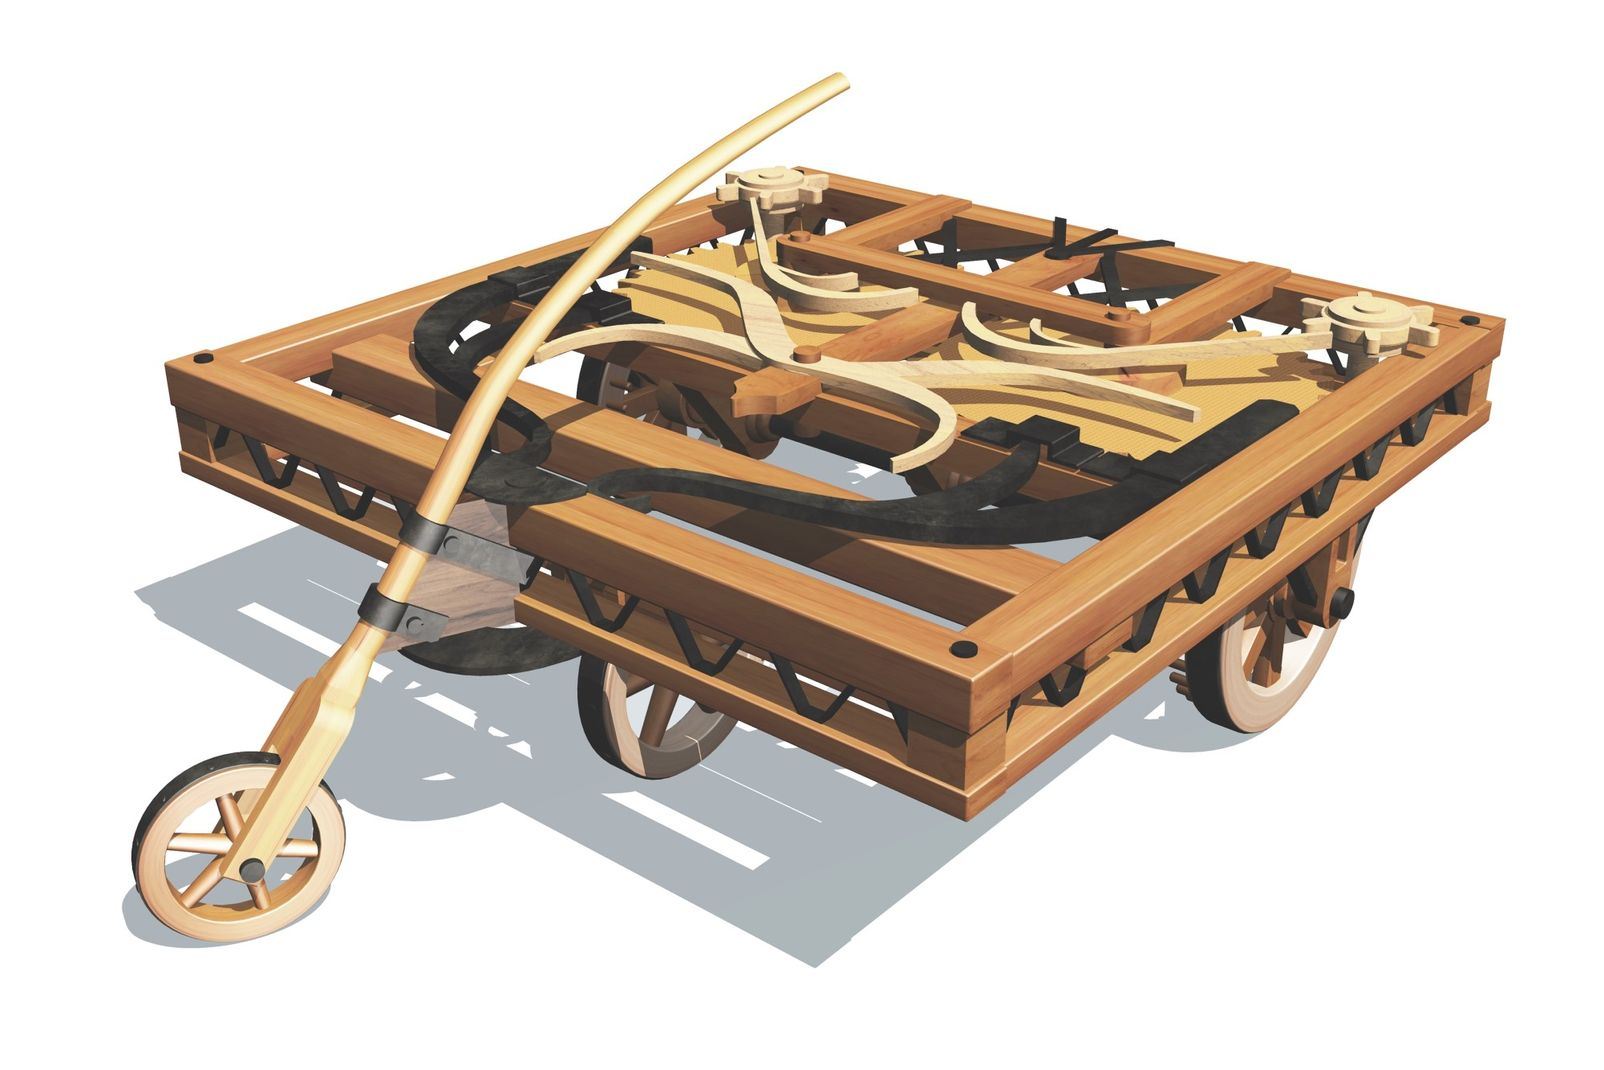
\includegraphics[width=0.35\textwidth]{ch1/figs/Vinci_car.jpg}
\caption{Model of autonomous car designed by Leonardo Da Vinci}
\label{fig:davinci_car}
\end{figure}

The field of robotics and autonomous systems has undergone significant evolution since the days of Leonardo, from rudimentary remote-controlled machines to highly advanced, AI-driven systems. These systems are no longer limited to following pre-defined paths or responding to simple commands. Modern autonomous robots can sense, analyze, and adapt to their environment, making decisions in real-time\cite{Samuels2023}. This leap in capabilities demands more sophisticated interactions between humans and robots, where ease of communication and control is vital for efficiency and safety. 

As we approach the Fifth Industrial Revolution (5IR), the focus shifts to a symbiotic relationship between humans and AI-powered robots, emphasizing workplace efficiency while maintaining a human-centric approach \cite{Samuels2023}. Augmented Reality (AR) plays a crucial role in this evolution, bridging the gap between humans and machines in areas such as manufacturing, healthcare, and human-robot interaction (HRI) \cite{Dalle2021}.

In the context of autonomous systems, fiducial markers (e.g., ARToolKit, AprilTags, ArUco) have become integral to robotics and AR applications. These markers facilitate robot navigation, environmental mapping, and interaction zone definition. The choice of marker system depends on specific application requirements, available computational resources, and desired accuracy.

The integration of AR and fiducial markers in robotics enhances perception, navigation, and interaction capabilities, pushing the boundaries of human-robot collaboration and making autonomous robots more adaptable and intelligent.





%@@@@@@@@@@@@@@@@@@@@@@@@@@@@@@@@@@@@@@@@@@@@@@@@@@@@@@@@@@@@@@@@@@@@@@@@@@@@@@@@@@@@@@@@@@@@@@@@@@@@@@
\section{\label{sec:probdesc}Problem Description}

As robots continue to evolve so does our demand for more intuitive and seamless interaction with these robots. Traditional control methods often fall short when it comes to offering the flexibility and situational awareness needed to integrate robots effectively into dynamic, real-world environments. This project addresses several key challenges in the domain of mobile robot control and environmental interaction:

\begin{enumerate}
    \item \textbf{Limited Contextual Awareness}: Current remote-controlled robots often operate with minimal understanding of their surroundings, leading to inefficient navigation and potential safety hazards in complex environments.
    \item \textbf{Inflexible Control Mechanisms}: Many existing robot control systems rely on fixed command sets that do not adapt to changing environmental conditions or task requirements, limiting their versatility and usability.
    \item \textbf{Absence of Dynamic Task Assignment}: Most mobile robots are pre-programmed for specific tasks and lack the ability to receive and interpret new instructions or environmental cues on the fly.
    \item \textbf{Integration Challenges}: Incorporating augmented reality (AR) elements into robotic systems presents technical challenges in terms of real-time processing, accurate marker detection, and seamless information overlay.
\end{enumerate}


%@@@@@@@@@@@@@@@@@@@@@@@@@@@@@@@@@@@@@@@@@@@@@@@@@@@@@@@@@@@@@@@@@@@@@@@@@@@@@@@@@@@@@@@@@@@@@@@@@@@@@@
\section{\label{sec:objectives}Objectives}

The primary objective of this project is to improve human-robot interaction (HRI) by integrating Augmented Reality (AR) technology with mobile robotics. Using AR and ArUco visual markers along with object detection measures, the robot will navigate and perform tasks in a more intuitive, human-centered way, enhancing both user experience and robot context-awareness.

This project focuses on developing a system that enables visual-based, real-time communication between the user and the robot. Through AR-enhanced interfaces and marker detection, the robot will perform context-aware tasks, with specific "control zones" triggering robot behaviors, and providing real-time AR feedback to the user.

\subsection{Main Objectives}
\begin{enumerate}
	\item \textbf{Control Zones Development}: AR-based zones will control robot behaviors, such as speed, task initiation, and directional changes, based on the detection of visual markers.
	\item \textbf{Real-time Dynamic Instructions}: The robot will use ArUco markers for real-time commands, allowing it to navigate, execute tasks, and respond to environment-specific instructions.
	\item \textbf{Environmental Mapping and Interaction}: Using visual markers, the robot will map its environment, track landmarks, avoid obstacles, and interact with objects.
	\item \textbf{Enhanced User Engagement}: AR will allow users to visually monitor and guide the robot in real-time, creating a more interactive and immersive user experience.
\end{enumerate}

\subsection{Secondary Objectives}

Additionally, two autonomous features will improve robot autonomy:
\begin{enumerate}
	\item \textbf{Object Avoidance}: The robot will detect specific markers and avoid obstacles by maintaining a defined safe distance (e.g., 20 cm).
	\item \textbf{Wheel Slip Detection}: The robot will detect terrain changes that may cause wheel slip and adjust its behavior based on power draw characteristics.
\end{enumerate}


\section{\label{sec:terms}Terms of Reference}

The system requirements, established through research, discussions with the supervisor, and analysis of the intended user environment, guide both the technical implementation and user experience. Key requirements include operating in AR-defined control zones, integrating dynamic instructions based on ArUco marker detection, environmental mapping using visual markers, providing real-time visual feedback, implementing object avoidance functionality, and detecting wheel slip events.

To meet these requirements, the system will implement several functionalities, including AR-based control zones, real-time ArUco marker processing, visual marker-based environmental mapping and obstacle avoidance, AR-based visual feedback for operators, object avoidance behavior, and wheel slip detection. Testing procedures have been outlined to ensure the system meets these requirements and functionalities, with specific sub-tests designed to check each function and requirement individually.


\section{\label{sec:scope}Scope and Limitations}

This project was conducted under several significant constraints that shaped the scope of the research and development process. These constraints were primarily due to limitations in time, budget, and available resources, which directly impacted the scale of the implementation and the range of features that could be developed.

The project had a total budget of R2000, which restricted the procurement of high-end components and forced the use of readily available, cost-effective hardware. Additionally, the project timeline was set at three months, limiting the ability to explore more advanced functionalities and requiring a focused approach to key objectives. These constraints influenced both the design and testing phases of the project.

Furthermore, ethical considerations were taken into account, particularly in ensuring that no invasive or harmful testing methods were used. The project did not involve human or animal subjects, which helped to avoid potential ethical conflicts and the need for additional approvals.

Despite these limitations, the project successfully demonstrated the integration of AR in human-robot interaction. While the constraints limited the full realization of more advanced features, the focused approach allowed the core objectives to be met within the available resources and timeline. Further development could build upon this foundation to explore more complex functionalities and broader applications.


\section{\label{sec:plan_of_development}Plan of Development}

This thesis is structured into seven chapters, each focusing on different aspects of the research and development process. The chapters build upon each other to present a coherent narrative from the conceptual framework to the implementation, testing, and conclusions of the project.

\textbf{Chapter 2: Literature Review}

Chapter 2 discusses the foundational technologies, theories, and techniques that underpin this project. It provides an overview of the state of the art in human-robot interaction (HRI), mobile robotics, and the use of Augmented Reality (AR) in robotics. 

\textbf{Chapter 3: Methodology}

Chapter 3 presents the research methodology used for this project. It provides detailed explanations of the procedures, experimental setups, and tools used for the development and testing of the system.

\textbf{Chapter 4: Prototype Design}

Chapter 4 focuses on the design of the system. It provides details on the hardware and software design choices, discussing how the various subsystems (e.g., AR integration, control zones, and dynamic instructions) were conceived and implemented. 

\textbf{Chapter 5: Modular Testing}

Chapter 5 Describes the testing process, including independent module testing, subsystem combinations testing, and the full integration phase. It describes how each individual system in the project (hardware and software) was tested.
 

\textbf{Chapter 6: Results and Analysis}

Chapter 6 presents the results obtained from the overall system. These results will showcase how the robot interacted with AR markers and control zones, as well as its performance in dynamic environments. Data from the acceptance tests will be analyzed to assess the system’s functionality and its success in meeting the project’s objectives.

\textbf{Chapter 7: Conclusion}

Chapter 7 concludes the thesis by reflecting on the overall project, summarizing the key findings, and discussing the implications of the results. It will cover the challenges faced during the project, how they were addressed, and potential areas for improvement. 


